\section{Design of estimators}

\subsection{ML and MAP estimators}

We define the maximum likelihood estimator (ML) as
\begin{equation}
\hat s_{\text{ML}} = \arg\max_{s} p_{{\bf X}|S}({\bf x}|s)
                   = \arg\max_{s} \ln(p_{{\bf X}|S}({\bf x}|s))
                    \label{ec:est_ML}
\end{equation}

It is important to emphasize that the maximization of $p_{{\bf X}|S}({\bf x}|s)$ has to be done with respect to the value of $s$, which is not the variable for which this probability function is defined. %Note that in the estimator definition alternatively includes  the use of the logarithm function (or some other with similar properties) and its use does not affect in any case the value resulting from maximization.

On the other hand, we define the maximum a posterior estimator (MAP) as
\begin{equation}
\hat s_{\text{MAP}} = \arg\max_{s} p_{{S|\bf X}}(s|{\bf x})
                   = \arg\max_{s} \ln(p_{{S|\bf X}}(s|{\bf x}))
                   \label{ec:est_MAP}
\end{equation}

in this case, maximization is performed on the same variable of the distribution that is being maximized. 

Note that both \eqref{ec:est_ML} and \eqref{ec:est_MAP} alternatively include the use of the logarithm function. This is done by practical reasons, since for the maximization of either the likelihood or the posterior of $S$ it may be useful to introduce an auxiliary function that simplifies the analytical form of the function and, since the logarithm function is defined for every positive value of its argument and is strictly increasing, it implies that if $p_{S|{\bf X}}(s_1|{\bf x}) > p_{S|{\bf X}}(s_2|{\bf x})$, then also $\ln p_{S|{\bf X}}(s_1|{\bf x}) > \ln p_{S|{\bf X}}(s_2|{\bf x})$). So, the introduction of the logarithm function will be useful when the likelihood or the a posterior  present products or exponentials, as it will transform products into sums and it will cancel exponentials. In this way, the maximization process can be simplified considerably.

If we compare both estimators, the ML estimator uses as statistical the likelihood of $S$ (a distribution which models the generation of the observations), whereas the MAP estimator uses the posterior distribution of $S$ (characterizes the behaviour of $S$ for any observed value), so the MAP estimator has a more complete information of the variable to be estimated. Nevertheless, the ML estimation does not require the definition of probability densities on the variable to be estimated (a prior or posterior distribution of the $S$ are not needed). Therefore, the use of the ML estimator is often used (or it is more appropriated) when such information is not available.

The ML estimator coincides with the MAP when $S$ has a uniform distribution in a range of values and, therefore, the application of the ML estimator in the absence of information about the a prior distribution of $S$ is equivalent to assuming uniformity in $S$ and applying the MAP estimator. To check this equivalence, one need only consider the relationship between the likelihood and the posterior distribution of $S$ by means of the Bayes Theorem,
$$ \hat s_{\text{MAP}} = \arg\max_{s} p_{{S|\bf X}}(s|{\bf x}) =  \arg\max_{s} \frac{p_{{\bf X}|S}({\bf x}|s) p_S(s)} {p_{\bf X}({\bf x})} $$
Since $p_{\bf X}({\bf x})$ does not depend {on $s$} and we are assuming that $p_S(s)$ is constant, we get:
$$ \hat s_{\text{MAP}} = \arg\max_{s} p_{{\bf X}|S}({\bf x}|s) = \hat s_{\text{ML}}$$
That is, the value of $s$ that maximizes the posterior has to coincide with the one that maximizes likelihood.



%%%%%%%%%%%%%%%
\begin{example}[Estimation ML]
\label{ex:est_ML_varaleat}
We want to estimate the value of a random variable $S$ from an observation $X$ statistically related to it. For the design of the estimator, only the likelihood of $S$ is known, which is given by
\begin{equation}
p_{X|S}(x|s) = \frac{2 x}{(1 - s)^2},\;\; 0<x<1-s,\;\; 0<s<1
\end{equation}
Given the available statistical information, it is decided to construct the ML estimator of $S$. For this purpose, the previous likelihood should be maximized. Such likelihood is a probability density function of $X$ as represented in Figure \ref{fig:est_ML_caso1}(a), where it is verified that the integral of this function with respect to $x$ is unitary. However, to carry out the maximization that allows to find $\hat s_{\text ML}$ it is more useful to represent this likelihood as a function of $s$ (Fig.\ref{fig:est_ML_caso1}(b))\footnote{Note that the integral with respect to $s$ of $p_{X|S}(x|s)$ will not generally be the unit, since this function does not constitute a probability density of $S$.}. From this graphic representation it is evident that the estimator is
$$\hat s_{\text{ML}} = 1 - x$$
or, alternatively, if we consider the application of the estimation function on the random variable $X$ instead of on a specific value of it,
$$\hat S_{\text{ML}} = 1 - X$$

%%%%%%%%%%%%%%
\begin{figure}[t]
  \begin{center}
  \begin{tabular}{cc}
    %\epsfig{file=Figures/px_s_funcionx, width=6cm} 
    \includegraphics[width=6cm]{Figures//px_s_funcionx.png} &
   % \epsfig{file=Figures/px_s_funcions, width=6cm} \\ 
   
   \includegraphics[width=6cm]{Figures//px_s_funcions.png}\\
    (a) & (b)
  \end{tabular}
    \caption{Representation of the likelihood distribution of the exercise \ref{ex:est_ML_varaleat} as a function of $x$ and $s$.}
    \label{fig:est_ML_caso1}
  \end{center}
\end{figure}
%%%%%%%%%%%%

\end{example}\vspace{0.4cm}
%%%%%%%%%%%%%


{
%%%%%%%%%%%%%%%
\begin{example}[Estimation MAP]
Considering that  
\begin{equation}
p(s|x) = \frac{1}{x^2} s \exp\left(-\frac{s}{x}\right), \qquad  x\ge 0, s \ge 0
\end{equation}
The MAP estimator can be computed maximizing
\begin{equation}
\ln(p(s|x)) = -2\ln(x) + \ln(s)-\frac{s}{x}, \qquad  x\ge 0, s \ge 0
\end{equation}
Since $\l(p(s|x))$ tends to $-\infty$ around $s=0 $ and $s=\infty$, its maximum must be at some intermediate point with zero derivative. Deriving respect to $s$ results in
\begin{equation}
\left.\frac{\partial}{\partial s} \ln p(s|x)\right|_{s=\hat{s}_\text{MAP}} = \frac{1}{\hat{s}_\text{MAP}} - \frac{1}{x} = 0, \qquad  x\ge 0, s \ge 0
\end{equation}
Thus,
\begin{equation}
\hat{s}_\text{MAP} = x
\end{equation}
\end{example}\vspace{0.4cm}}
%%%%%%%%%%%%%


\subsection{Bayesian design of estimators}

It is worth asking, for a given cost and distribution, which is the best possible estimator. We can find this out by taking into account that, generally speaking, the average cost can be expressed as
\begin{align}
\label{ec:coste_medio}
\mathbb{E}\{c(S,\hat S)\} 
& = \int_{\bf x} \int_s c(s,\hat s) p_{S|{\bf X}}(s|{\bf x}) ds\;p_{\bf X}(\bf x) d{\bf x} = \nonumber\\
& = \int_{\bf x} \mathbb{E}\{c(S,\hat s)|{\bf X} = {\bf x} \} p_{\bf X}(\bf x) d{\bf x}.
\end{align}

The last line of this equation shows that a strategy for minimizing the overall estimation cost consists of minimizing the mean cost for each possible value of the observation vector,  $\mathbb{E}\{c(S,\hat s)|{\bf X} = {\bf x} \}$, which we will refer to as mean posterior cost or mean cost given ${\bf X}$. Therefore, both strategies (minimization of the expected cost for all $S$ and $\bf X$, or conditioned to the value of $\bf X$) are in principle equivalent in order to obtain the optimal estimator associated with a given cost function.

The Bayesian Estimator associated with a cost function is defined {as} that which minimizes \eqref{ec:coste_medio}, that is:

\begin{equation}
\label{ec:est_bayesiano}
{\hat s}^* = \arg\min_{\hat s}\;\mathbb{E}\{c(S,\hat s)|{\bf X} = {\bf x} \}
\end{equation}

where $\hat s^*$ is the Bayesian Estimator. According to our previous discussion, the Bayesian Estimator also minimizes the expected cost in a global sense, i.e., for all $S$ and ${\bf X}$. Note, however, that for your design the expression \eqref{ec:est_bayesiano} is more useful than the direct minimization of the overall cost.

\begin{equation}
\mathbb{E}\{c(S,\hat S)\} = \int_{\bf x} \mathbb{E}\{c(S,\hat s)|{\bf X} = {\bf x} \} p_{\bf X}(\bf x) d{\bf x}
\end{equation}

since calculating the integral in ${\bf x}$ would require knowing beforehand the relationship between $\hat s$ and $\bf x$, which is precisely the objective of the estimator design problem.

%%%%%%%%%%%%%%%
\begin{example}[Calculation of a minimum mean square error estimator]
\label{CalculoECM2}
Following the example \ref{CalculoECM}, we can calculate the posterior distribution of $S$ through
\begin{equation}
p_{S|X}(s|x) = \frac{p_{S,X}(s,x)}{p_{X}(x)}. 
\end{equation}
Knowing that
\begin{equation}
p_{X}(x) = \int_0^1 p_{S,X}(s,x) ds = \int_0^x \frac{1}{x} ds = 1,
\end{equation}
we obtain
\begin{equation}
p_{S|X}(s|x) = \left[
\begin{array}{ll}
\frac{1}{x}, & \qquad 0<s<x<1 \\
0,           & \qquad \text{otherwise}
\end{array}
\right.
\end{equation}
The mean cost given the observation will be given by
\begin{align}
\mathbb{E}\{c(S,\hat s)|X=x\} 
   &= \mathbb{E}\{(S-\hat s)^2|X=x\} \nonumber\\
   &= \int_0^1 (s-\hat{s})^2 p_{S|X}(s|x) ds   \nonumber\\
   &= \frac{1}{x} \int_0^x (s-\hat{s})^2 ds   \nonumber\\
   &= \frac{1}{x} \left(\frac{(x-\hat{s})^3}{3} + \frac{\hat{s}^3}{3} \right)    \nonumber\\
   &= \frac{1}{3}x^2 - \hat{s} x + \hat{s}^2. 
\label{Est:ECMsx}
\end{align}

As a function of $\hat{s}$, the mean cost conditioned to the observation is a polynomial of second degree, whose minimum can be calculated immediately by derivation. Being
\begin{align}
\frac{d}{d\hat{s}} \mathbb{E}\{c(S,\hat s)|X=x\} 
   &= - x + 2 \hat{s} ,
\end{align}
the lowest mean quadratic error estimator will be
\begin{equation}
\label{eq:sopt_halfx}
\hat{s}^* = \frac{1}{2}x,
\end{equation}
which matches the estimator $\hat{S}_1$ from the example \ref{CalculoECM}. Therefore, $\hat{S}_1$ is the best possible estimator from the point of view of the mean square error.
\end{example}\vspace{0.4cm}
%%%%%%%%%%%%%

Based on \eqref{ec:est_bayesiano} we can conclude that, regardless of the cost to be minimized, the knowledge of the posterior distribution of $S$ given ${\bf X}$, $p_{S|{\bf X}}(s|{\bf x})$, is sufficient for the design of the Bayesian Optimal Estimator. As mentioned above, this distribution is often calculated from the likelihood of $S$ and its a prior distribution using the Bayes Theorem, which is in fact the origin of the denomination of these estimators.

%%%%%%%%%%%%%%%%%%%%%%%%%%%%%%%%%%%%%%%%%%%%%%%%%
\section{Common bayesian estimators}
%%%%%%%%%%%%%%%%%%%%%%%%%%%%%%%%%%%%%%%%%%%%%%%%%

This section presents some of the most commonly used Bayesian estimators. For their calculation, we will proceed to minimize the mean cost given $\bf X$ (posterior mean cost) for different cost functions.


%%%%%%%%%%%%%%%%%%%%%%%%%%%%%%%%%%%%%%%%%%%%%%%%%%%%%%%%%%%%%%
\subsection{Minimum Mean Squared Error estimator (MSE)}
The estimator of minimum mean squared error (MSE) is the one associated with the cost function $c(e) = e^2 = (s-\hat s)^2$, and therefore is characterized by 
\begin{align}
\label{ec:coste_medio_cuadratico}
\hat s_{\text{MSE}} 
  & = \arg\min_{\hat s} \; \mathbb{E}\{c(S,\hat s)|{\bf X} = {\bf x} \} = \\
  & = \arg\min_{\hat s} \int_s (s - \hat s)^2 p_{S|{\bf X}}(s|{\bf x}) ds
\end{align}

Figure \ref{fig:estimador_cuadratico} illustrates the design problem with the minimum mean squared error estimator. The mean posterior cost can be obtained by integrating in $s$ the function resulting from the product of the cost function and the posterior probability density of $S$. The argument for minimization is $\hat s$, which allows to move the graph corresponding to the cost function (represented with discontinuous stroke) so that the result of that integral is minimal.

%%%%%%%%%%%%%%
\begin{figure}[th]
  \begin{center}
    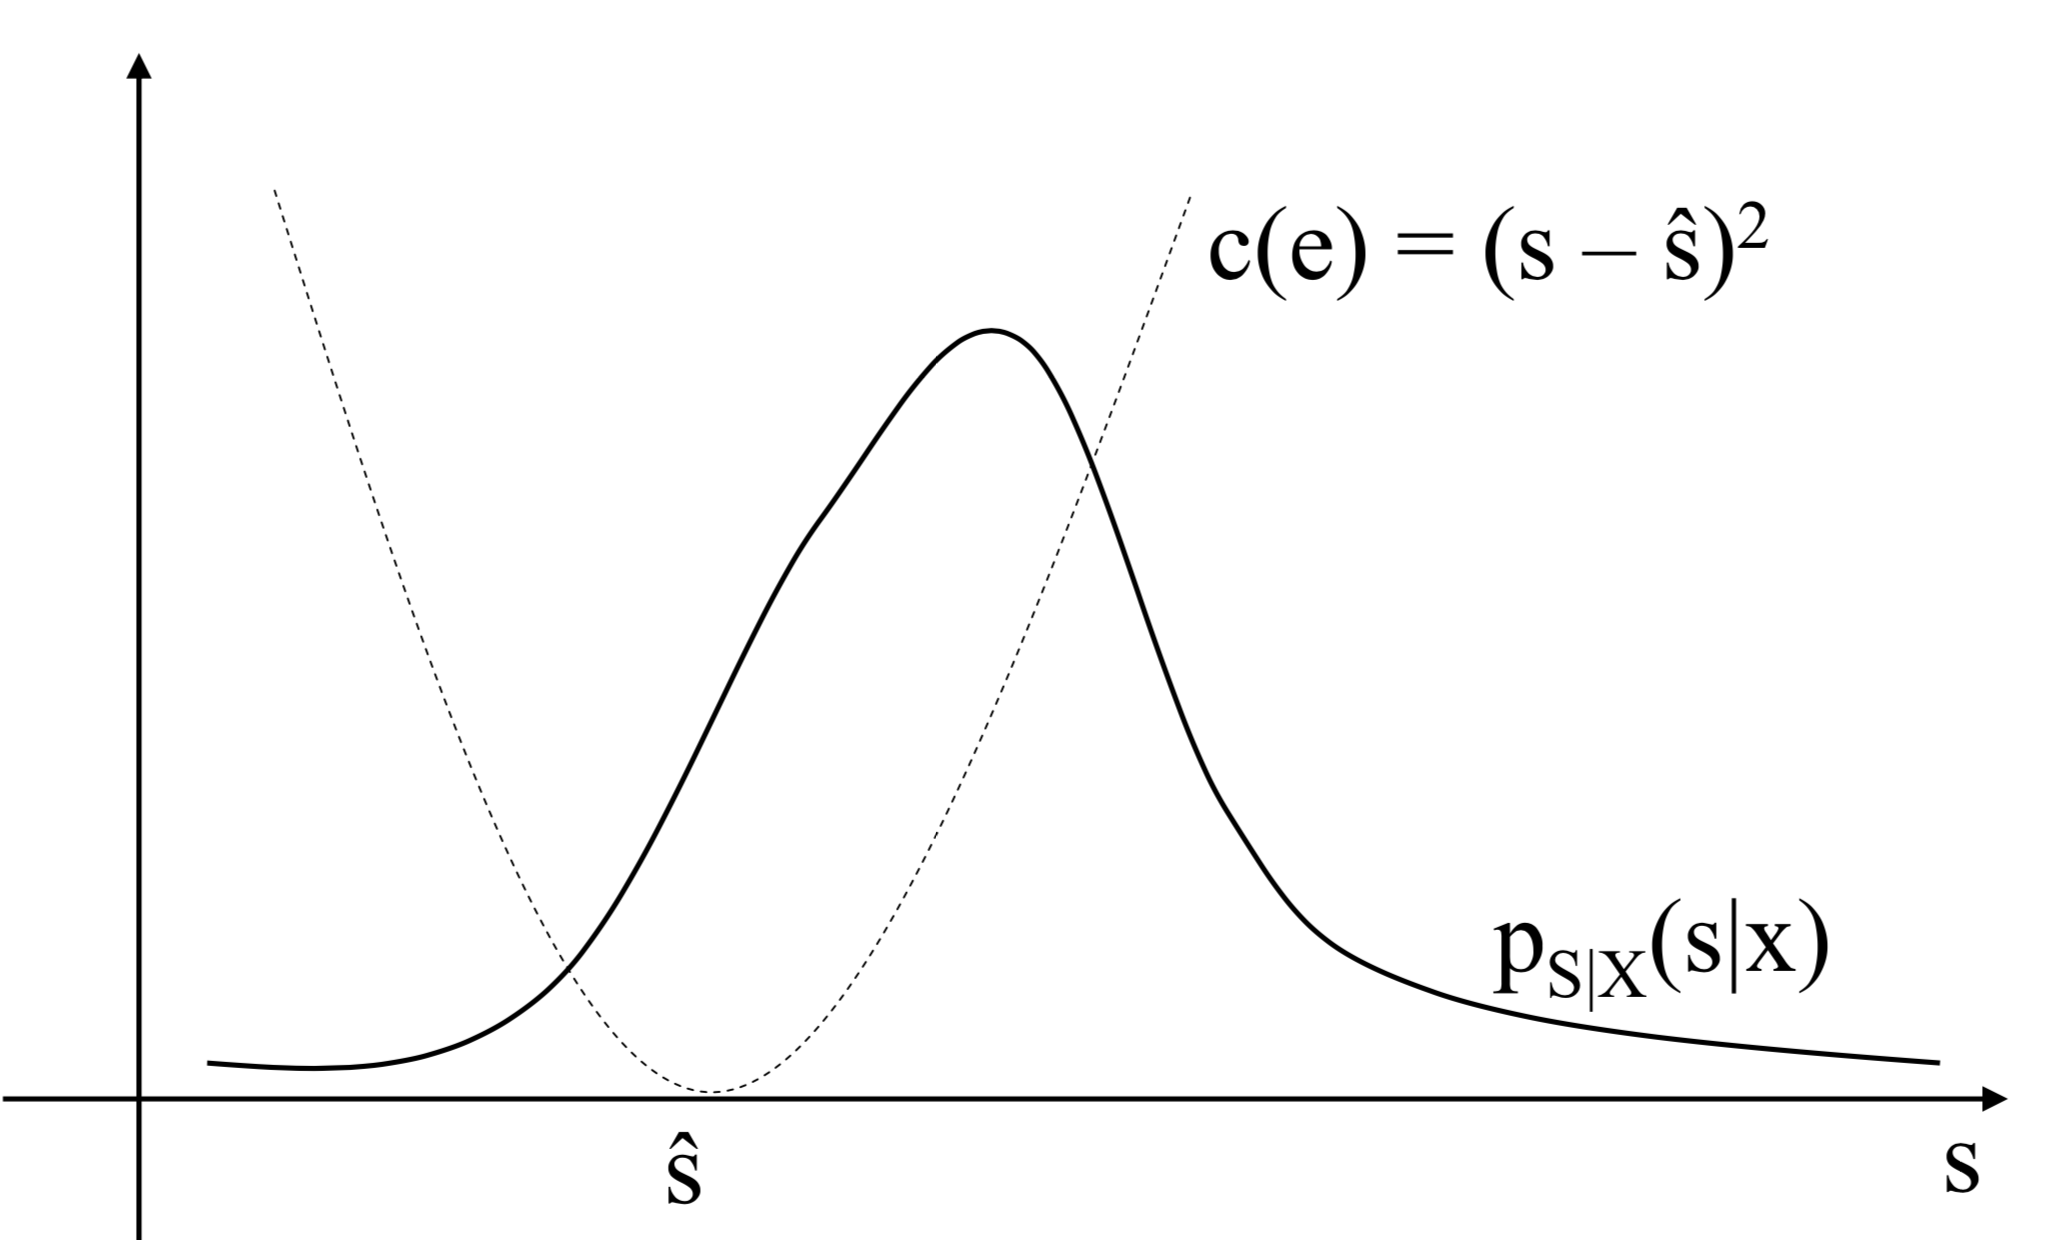
\includegraphics[width=10cm]{Figures//estimador_cuadratico.png}
    \caption{Graphical representation of the process of calculating the posterior mean for a generic value $\hat{s}$.}
    \label{fig:estimador_cuadratico}
  \end{center}
\end{figure}
%%%%%%%%%%%%

The value of $\hat s_{\text{MSE}}$ can be analytically obtained by taking the derivative of the posterior mean cost and equaling the result to 0. The calculation of the derivative does not pose any difficulty since the derivative and the integral can be commutated (it is integrated with respect to $s$ and is derived with respect to $\hat s$):
\begin{equation}
\label{ec:estimador_MSE}
\left.\frac{d \mathbb{E}\{(S-\hat s)^2| {\bf X}={\bf x}\}}{d \hat s}\right|_{\hat s = \hat s_{\text{MSE}}} = -2 \int_s (s - \hat s_{\text{MSE}}) p_{S|{\bf X}}(s|{\bf x}) ds = 0
\end{equation}


Bearing in mind that the integral in \eqref{ec:estimador_MSE} should be cancelled, and using the fact that $\int p_{S|{\bf X}}(s|{\bf x}) ds = 1$, it is easy to demonstrate that the minimum mean squared error estimator of $S$ is given by

\begin{framed}
\begin{equation}
\label{ec:estimador_MSE_final}
\hat s_{\text{MSE}} = \int s\;p_{S|{\bf X}}(s|x) ds = \mathbb{E}\{S|{\bf X} ={\bf x}\}
\end{equation}
\end{framed}

In other words, the minimum mean squared error estimator of $S$ is the mean of $S$ given $\bf X$ or the posterior mean of $S$ , i.e., the expected value of $p_{S|{\bf X}}(s|{\bf x})$.

%%%%%%%%%%%%%%%%
%\begin{exercise}
%Check that the expression \eqref{ec:estimador_MSE_final} actually constitutes a minimum of the given average cost {\bf X}, by calculating the second derivative of $\mathbb{E}\c(S,\hat s)|{bf X} = {\bf x}$.
%\end{exercise}
%%%%%%%%%%%%%%


%%%%%%%%%%%%%%%
\begin{example}[Straightforward calculation of the MSE estimator]
According to \eqref{ec:estimador_MSE_final}, minimum mean squared error estimator obtained in \ref{CalculoECM} can alternatively be obtained as follows

\begin{align}
\label{ec:estimador_MSE_final2}
\hat s_{\text{MSE}} = \int_0^1 s p_{S|X}(s|x) ds   
   = \int_0^x \frac{s}{x} ds 
   = \frac{1}{2} x
\end{align}
which coincides with \eqref{eq:sopt_halfx}.
\end{example}\vspace{0.4cm}
%%%%%%%%%%%%%



%%%%%%%%%%%%%%%%%%%%%%%%%%%%%%%%%%%%%%%%%%%%%%%%%%%%%
\subsection{Minimum Mean Absolute Deviation Estimator (MAD)}

In the same way as we have proceeded in the case of the estimator $\hat s_\text{MSE}$, we can calculate the estimator associated with the absolute deviation of the estimation error, $c(e) = |e| = |s - \hat s|$. This estimator, which we will refer to as the Mean Absolute Deviation (MAD), is characterized by

\begin{equation}
\label{ec:coste_MAD}
\begin{split}
\hat s_{\text{MAD}} & = \arg\min_{\hat s}\; \mathbb{E}\{|S - \hat s|~|{\bf X} = {\bf x} \} = \\
& = \arg\min_{\hat s} \int_s |s - \hat s|\;p_{S|{\bf X}}(s|{\bf x}) ds
\end{split}
\end{equation}


Again, it is simple to illustrate the process of calculating the posterior mean cost by overlapping on the same axes the cost expressed as a function of $s$ and the posterior distribution of the variable to be estimated (see Fig. \ref{fig:estimador_absoluto}). This representation also suggests the convenience of splitting the integral into two parts corresponding to the two slopes of the cost function:


\begin{equation}
\begin{split}
\mathbb{E}\{|S - \hat s|~|{\bf X} = {\bf x} \} &= \int_{-\infty}^{\hat s} (\hat s - s) \;p_{S|{\bf X}}(s|{\bf x}) ds + \int_{\hat s}^\infty (s - \hat s) \;p_{S|{\bf X}}(s|{\bf x}) ds \\
& = \hat s \left[ \int_{-\infty}^{\hat s} p_{S|{\bf X}}(s|{\bf x}) ds -  \int_{\hat s}^{\infty} p_{S|{\bf X}}(s|{\bf x}) ds\right] + \\
&\;\;\;\;\;\;\;\;\;\;\;\; + \int_{\hat s}^{\infty} s\;p_{S|{\bf X}}(s|{\bf x}) ds -  \int_{-\infty}^{\hat s} s \; p_{S|{\bf X}}(s|{\bf x}) ds
\end{split}
\end{equation}

%%%%%%%%%%%%%%
\begin{figure}[t]
  \begin{center}
  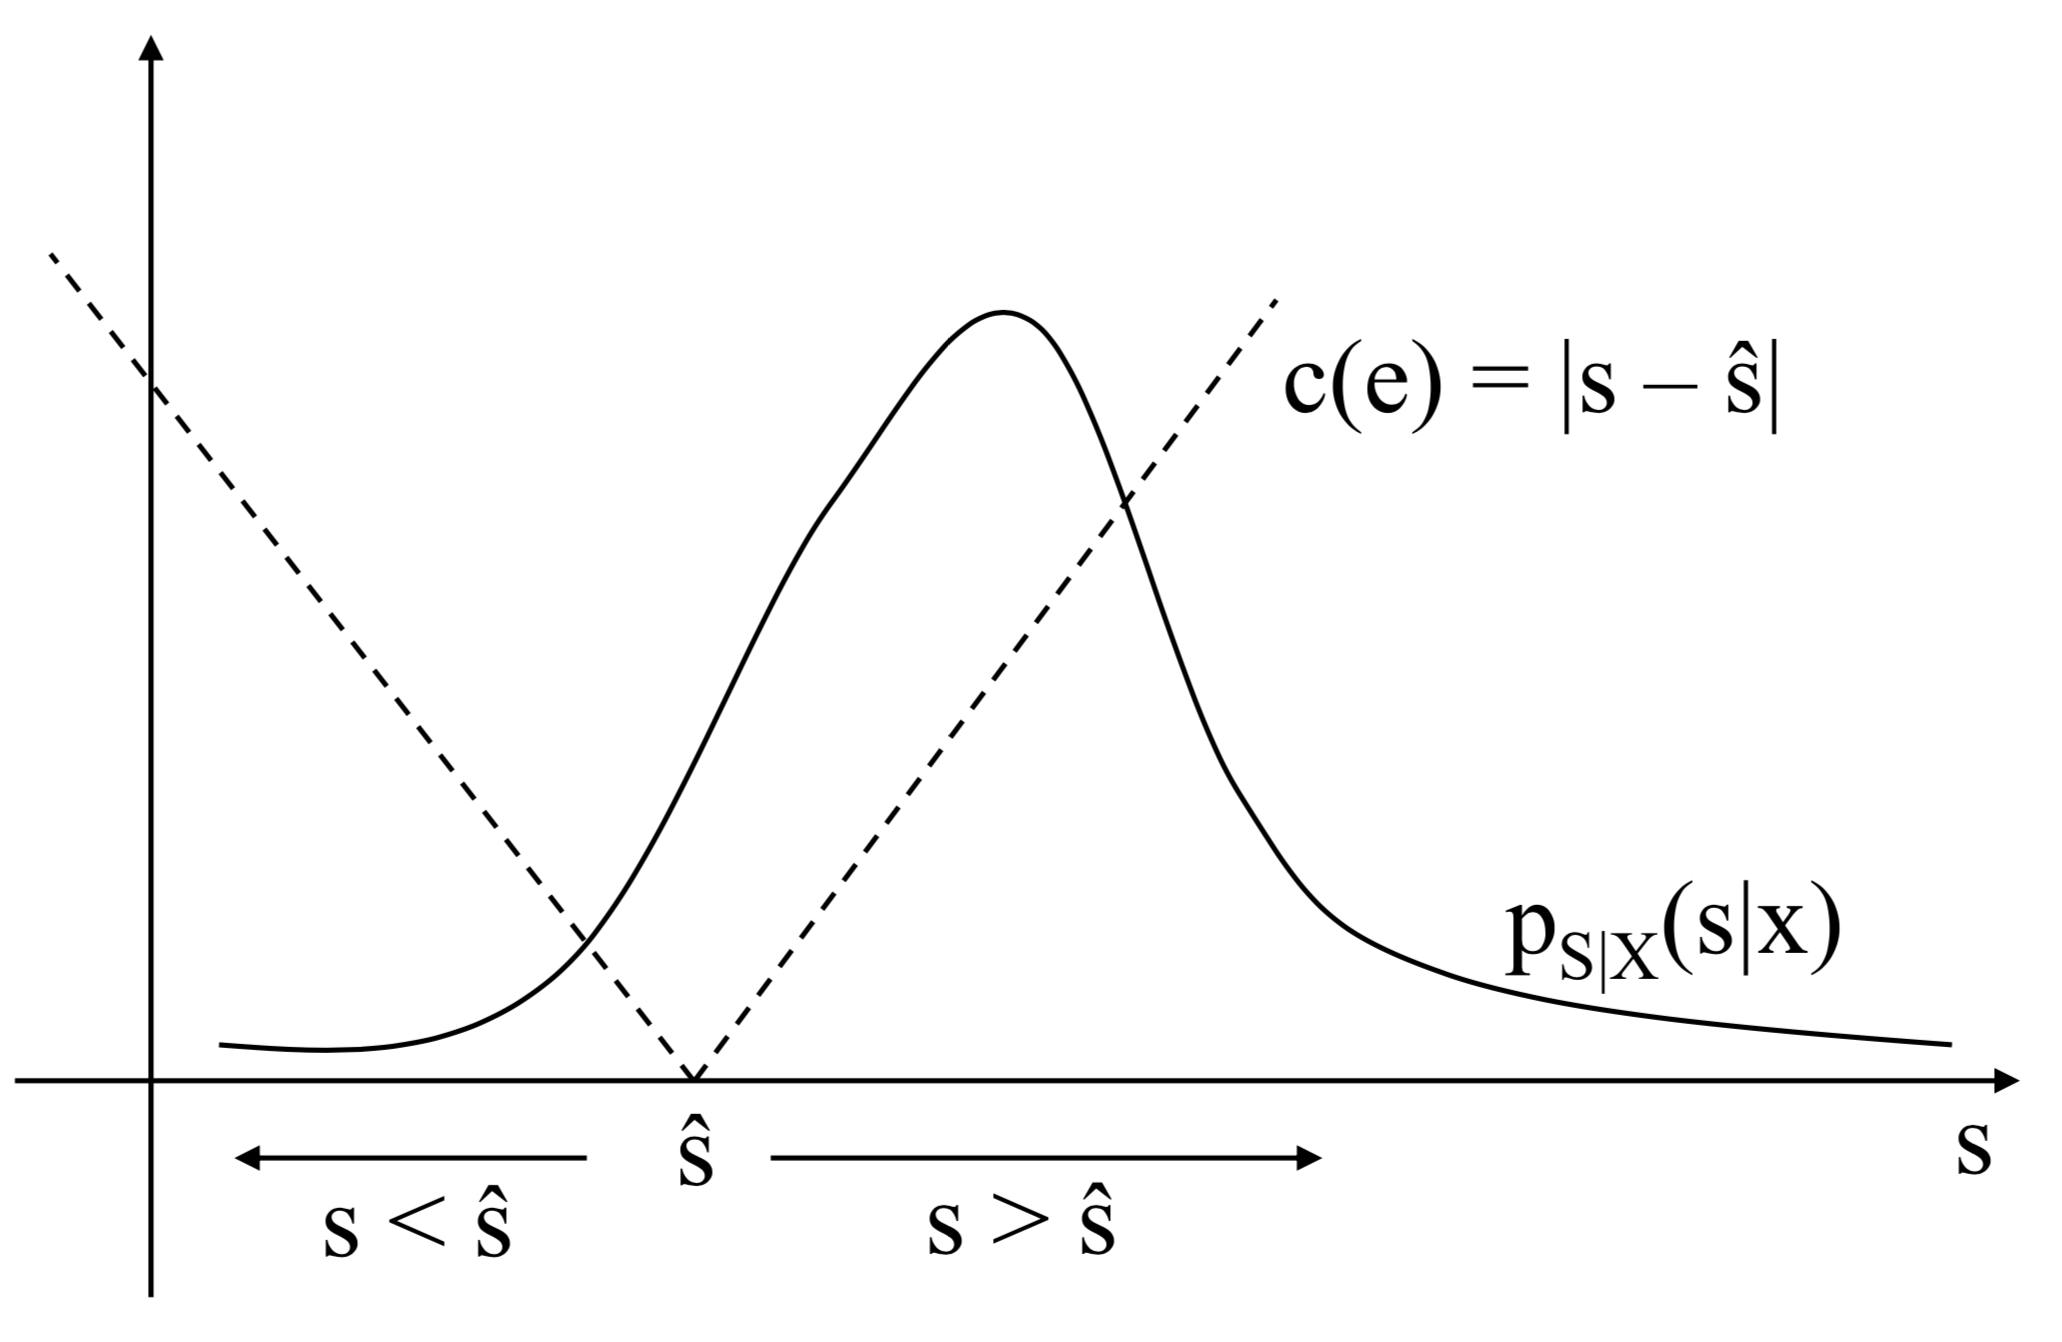
\includegraphics[width=10cm]{Figures//estimador_absoluto.png}
    \caption{Graphical representation of  the process of calculating the posterior mean absolute error for a generic value $\hat s$.}
    \label{fig:estimador_absoluto}
  \end{center}
\end{figure}
%%%%%%%%%%%%

The fundamental theorem of calculus\footnote{$\frac{d}{d x} \int_{t_0}^x g(t) dt = g(x)$.} allows us to obtain the derivative of the posterior mean cost as
\begin{equation}
\frac{d \mathbb{E}\{|S - \hat s|~|{\bf X} = {\bf x} \}}{d \hat s} = 2 F_{S|{\bf X}}(\hat s|{\bf x}) - 1
\end{equation}

where $F_{S|{\bf X}}(s|{\bf x})$ is the posterior distribution function of $S$ given ${\bf X}$. Since $\hat s_{\text{MAD}}$ represents the minimum of the mean cost, the previous derivative must be cancelled for the estimator, verifying that $F_{S|{\bf X}}(\hat s_{\text{MAD}}|{\bf x}) = 1/2$. In other words, the absolute minimum error estimator is given by the median of $p_{S|{\bf X}}(s|{\bf x})$:

\begin{framed}
\begin{equation}
\label{ec:estimador_MAD_final}
\hat s_{\text{MAD}} = \text{median}\{S|{\bf X} ={\bf x}\}
\end{equation}
\end{framed}

Remember that the median of a distribution is the point that separates that distribution into two regions that have the same probability, so the minimum mean absolute error estimator will verify that
{$$P\{S > \hat s_{\text{MAD}}\} = P\{S < \hat s_{\text{MAD}}\}$$}

{\begin{example}[Design of a Minimum Mean Absolute Deviation Estimator]

In the scenario of the example \ref{CalculoECM}, the a posterior distribution of $S$ given $X$ is uniform between 0 and $x$, the median of which is $x/2$. So,

\begin{align}
\label{ec:estimador_MSE_finalej}
\hat s_{\text{MAD}} = \frac{1}{2} x 
\end{align}

Note that, in this case, the MAD estimator matches the MSE obtained at \eqref{eq:sopt_halfx}. This is a consequence of the symmetry of the a posterior distribution. In general, both estimators do not have to coincide.

\end{example}\vspace{0.4cm}
}



